

\begin{frame}[ctb!]
  \frametitle{Extensions : Fracturation}
    \begin{minipage}{0.49\textwidth}
      \begin{figure}[h!]
        \includegraphics[width=\textwidth]{fracturesAB.eps}
        \label{fig:fracturesAB}
      \end{figure}
    \end{minipage}
    \hspace{.01cm}
    \begin{minipage}{0.49\textwidth}
      \begin{figure}[h!]
        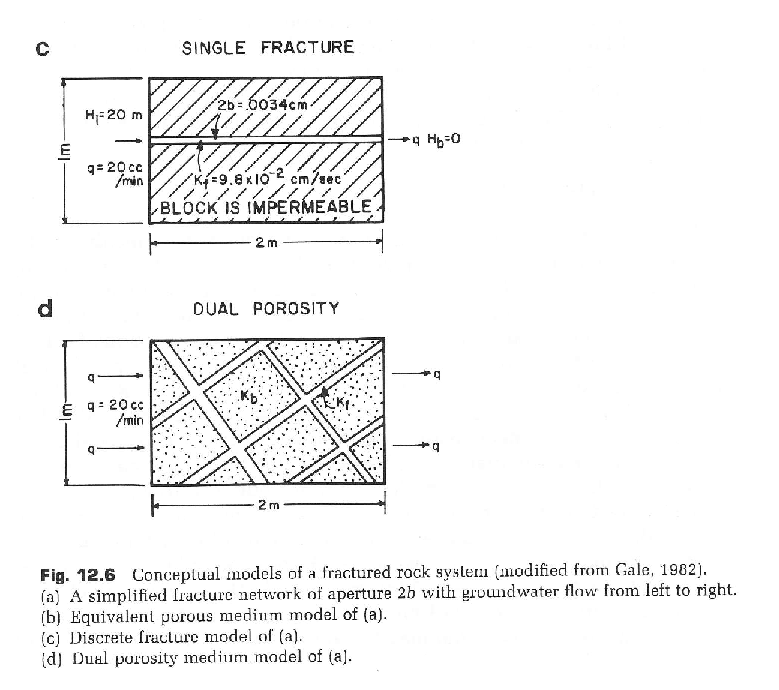
\includegraphics[width=\textwidth]{fracturesCD.eps}
        \label{fig:fracturesCD}
      \end{figure}
    \end{minipage}

  A dual continuum model will be implemented to more accurately represent 
  fractured host media such as granite \cite{anderson_applied_1992}.
\end{frame}


\begin{frame}[ctb!]
  \frametitle{Extensions : Sorption}
  \begin{figure}[h!]
      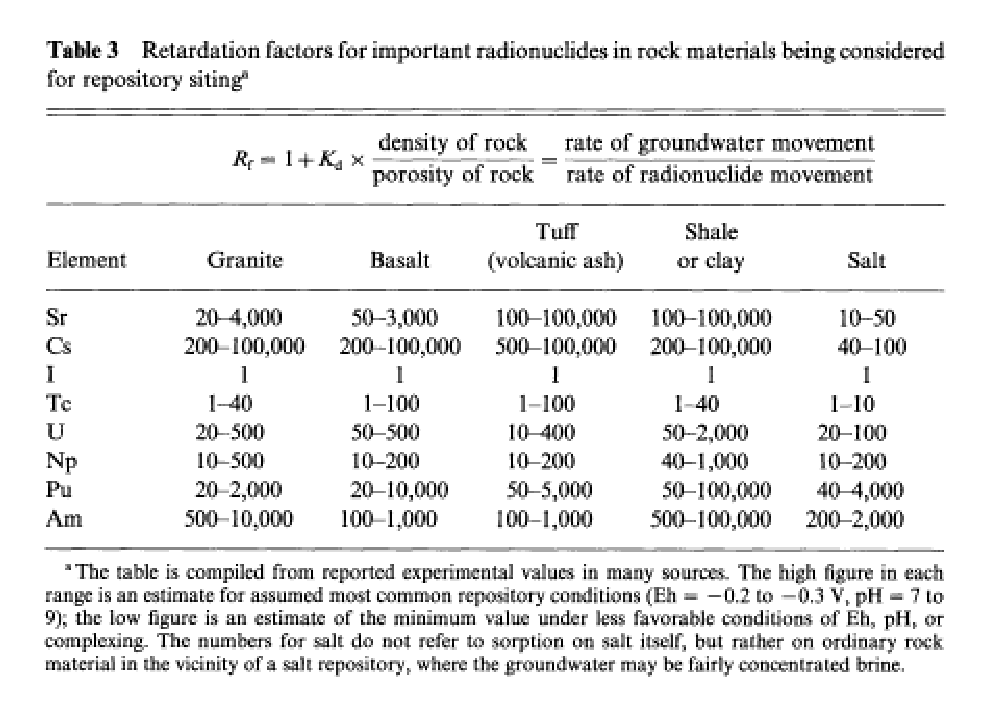
\includegraphics[height=.8\textheight]{sorptionKrauskopf.eps}
    \caption{Sorption will be modeled using retardation factors in the mixed 
    cell models \cite{krauskopf_geology_1988.}}
    \label{fig:sorptionKrauskopf}
  \end{figure}
\end{frame}


\begin{frame}[ctb!]
  \frametitle{Extensions : Coalescence}
  Salt and clay exhibit coalescent behavior under heat.
\end{frame}

